\begin{frame}{BCDI data analysis workflow}
    \begin{columns}
        \column[T]{0.48\textwidth}
        \begin{figure}
            \centering
            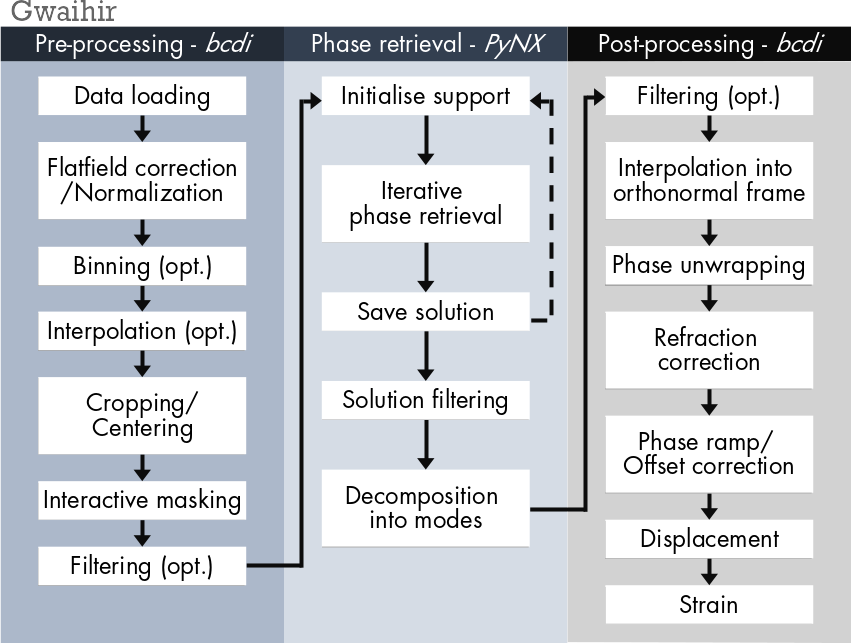
\includegraphics[width=\textwidth]{Figures/gwaihir/Packages.png}
            \caption{Flow chart of the main steps in the BCDI data analysis workflow.}
            \label{fig:Packages}
        \end{figure}
        
        \column[T]{0.48\textwidth}

        \pause
        
        \begin{figure}
            \centering
            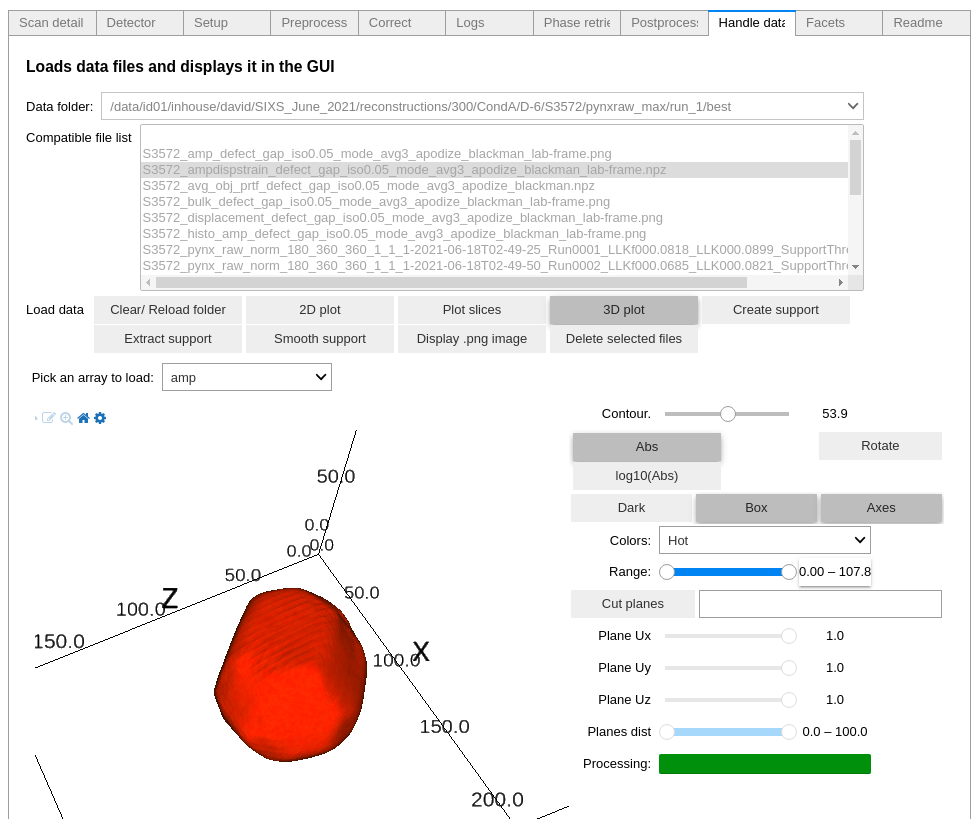
\includegraphics[width=\textwidth]{Figures/gwaihir/GUI_handle_tab.png}
            \caption{Data analysis is performed through interactive widgets.}
            \label{fig:GUI_handle_tab}
        \end{figure}

    \end{columns}

    \pause
    \begin{columns}
        \column[T]{0.03\textwidth}
        \vspace{-0.02cm}
        \begin{figure}[T]
            
\includegraphics[width=\textwidth]{Figures/gwaihir/GitHub-Mark-120px-plus.png}
        \end{figure}
        
        \column[T]{0.9\textwidth}
        \medskip
        GitHub repository (open access\footnotemark{}): \href{GitHub.com/Dsimonne/Gwaihir\#welcome}{GitHub.com/Dsimonne/Gwaihir\#welcome}
        
    \end{columns}
    
    \footnotetext{Gwaihir: Jupyter Notebook Graphical User Interface for Bragg Coherent Diffraction Imaging D. Simonne et al., (2022). J. Applied Crystallography (Volume 55, Part 4)}
\end{frame}